\documentclass[10pt,twocolumn]{article}
	
\usepackage{myfontstyle}
\usepackage{mypackages}
\usepackage{mymacros}
\usepackage{mycommands}

\begin{document}
\thispagestyle{fancy1}

%%% Title and Abstract------------------------
\twocolumn[
\begin{center}
	\hrule
	\vspace{3pt}
	% Title:
	{\sffamily\bfseries\Large
		Report for Laboratory Three: RC Circuit Response
	} \\
	{\color{gray}
		\vspace{3pt}
		\hrule
		\vspace{3pt}
	}
	{
		\hspace*{\fill}
		Austin Piper
		\hspace*{\fill}
		Alex Blakley
		\hspace*{\fill}
		Irfan Ahmed
		\hspace*{\fill}
%		Fourth Author    % uncomment these two lines if there's a fourth author
%		\hspace*{\fill}
	}\\
	\vspace{3pt}
	{\itshape
		\hspace*{\fill}
		Department of Mechanical Engineering, Saint Martin's University
		\hspace*{\fill} \\
		\hspace*{\fill}
		ME/EE 316---Mechatronics \& Measurements Laboratory
		\hspace*{\fill}
	}\\
	\vspace{3pt}
	{
		\hspace*{\fill}
		\today{} % today's date ... can type manually instead
		\hspace*{\fill}
	}
	\vspace{3pt}
	{\color{gray}\hrule}
%	\vspace{2pt}
\end{center}
% Abstract:
\begin{adjustwidth}{1.5in}{1.5in}
{\small
\noindent\textbf{Abstract.} \hspace{1em}
	The purpose of this lab was to view and measure the response of the voltage across a capacitor in a RC circuit. After building the circuit on a breadboard we sent 1 volt across the completed circuit and we used the myRIO microcontroller in order to record the results. The output voltage and resulting graphs can be used to find the time constant.
}
\end{adjustwidth}
\vspace{9pt}
\hrule
\vspace{1\baselineskip}
]

%%% Body -------------------------

\section{Introduction} 
\label{sec:introduction}

There are many variations of circuits used in the world of electronics in order to accomplish and power useful machines. The common RC circuit is used in devices like pacemakers, noise cancelling products, and timing circuits. These types of circuits are used because they can filter signals, blocking some and allowing others to pass through and therefore they are effective in their usage. 

In this lab, we built a basic RC circuit on a breadboard with a single 100 kΩ resistor and a 10 µF capacitor. We hooked up the myRIO to the breadboard and, with the full circuit completed and grounded using jumper wires, we applied a DC voltage across the capacitor and the measurements were taken of both the source voltage and output voltage.  The advantage of using the myRIO is that we could pair this technology with the LabVIEW program in order to have a graph drafted, in real time, of both of the data streams we require in order to deepen our understanding of how the RC circuit reacts to a constant voltage over time. 

\begin{figure}
  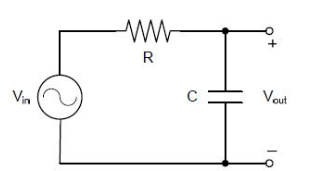
\includegraphics[width=\linewidth]{/figures/RC_Circuit.PNG}
  \caption{An RC Circuit}
  \label{fig:rc1}
\end{figure}

Figure \ref{fig:rc1} An RC Circuit

\section{Materials and Methods}

This experiment started with the building of a circuit that had a 100 kΩ resistor and a 10 µF capacitor in series using a breadboard and jumper wires. Using a multimeter, both the capacitor and resistor were measured in order to ensure they, indeed, had the desired value of capacitance and resistance we needed for the experiment. After the myRIO was connected to our circuit we then began setting up the LabVIEW program in order to both control the source voltage supplied across the capacitor and to measure the output voltage over time. Using LabVIEW, we were able to grab the data and create a graph that showed both of the aforementioned voltages after about 6 time constants (6RC).
\section{Results}
\label{sec:results}

``To write the results section, use the figures and tables as a guide. Start by outlining, in point form, what you found, going slowly through each part of the figures. Then take the points and group them into paragraphs, and finally order the points within each paragraph. Present the data as fully as possible, including stuff that at the moment does not quite make sense.

``Verbs in the results section are usually in the past tense. Only established scientific knowledge is written about in the present tense, `the world is round,' for example. You cannot presume that your own data are part of the body of established scientific knowledge, and so when you describe your own results, use the past tense, `a band of 1.3 KB was seen,' for example. There are, however, exceptions to this general rule. It is acceptable to say, `Table 3 shows the sizes of the DNA fragments in our preparation.' It is also acceptable to say, `In a 1991 paper, Ebright and coworkers used PCR to mutagenize DNA.' \ldots

``Some readers begin by scanning the figures first. The figures, with the legends, should provide a self-explanatory overview of your data. Decide what the data show, then create figures which highlight the most important points of your paper.

``Tables are used to present repetitive data that is numerical. Graphs or illustrations, collectively called figures, are used to present numerical trends, raw data (like a picture of a gel), or a model that explains your work.

``When you prepare your figures and tables, keep in mind that it is significantly more expensive for journals to publish figures and tables than text, so try to present the data in a way that is worthy of such added expense.''

\section{Discussion}

``This is the section of the paper for you to show off your understanding of the data. You should summarize what you found. Explain how this relates to what others have found. Explain the implications.''

\section{Author Contributions}

You are required to describe each member's contributions to the laboratory exercise and report.

%%% References -------------------------

\bibliographystyle{plainnat}
\bibliography{report}

%%% Appendices -------------------------

\appendix

\section{Appendix: \LaTeX{} Tutorial}\label{sec:latex}

I'm going to teach you how to use \LaTeX{} a little bit. Like how to cite a source, insert a graphic, and build tables. Follow along in the \texttt{report.tex} file.

{\bfseries\color{red} Do not use this appendix as any sort of template for the report! Equations, figures, and tables should appear in the body of the report.} Delete this appendix before submitting your report.

\subsection{Citing a Source}

Let's cite a source. The source must be already saved as a BibTeX file (\texttt{.bib}) in the same directory as the \texttt{.tex} document. I have already created a sample \texttt{report.bib} file. (If you want to add and remove sources to this file, you may use a reference manager like BibDesk on a Mac or JabRef on a PC.)

The next step is to cite the source, inline~\citep{Rowell1997}. And I can easily cite another reference~\citep{Ciesielski1997}.

\subsection{Equations}

Equations should appear in the body of the report, especially in the Introduction (\autoref{sec:introduction}), when describing your theoretical predictions. An equation should be part of a complete sentence.

Here are some examples.

We now see that
\begin{align}
	x = 1 .
\end{align}

Somehow, the following impossible equation hold:
\begin{align} \label{eq:int}
	\int_0^t x_2 \sin{x} dx = 
	\begin{bmatrix}
		1 & 0 & 8 \\
		0 & x^7 \\
		7 &
	\end{bmatrix} .
\end{align}
We now see that 
\begin{align}
	\bm{x} = \bm{\alpha} 
    \left( 
    	\left(
        	\frac{2}{3}
        \right) + 
        \frac{5}{6} 
    \right) , 
\end{align}
where $\bm{\alpha}$ is the coefficient of stupidity.

And this works too: $\frac{\partial x}{\partial y}$ .

\begin{subequations}
\begin{align*}
	x &= 2 y & \text{(where $x>2$)} \\
	y &= 4 x + 8 &
\end{align*}
\end{subequations}

Later, you could refer to the equation \autoref{eq:int}.

Or you could do it multiple times: \autoref{eq:int}.

\subsection{Figures}
It is easy enough to add a figure. In the subdirectory \texttt{figures}, I placed a file \texttt{data.pdf}. If we want to include it in the document, we use the following commands.



\subsection{Tables}
Tables can be a pain in \LaTeX{}. Here's a simple table.

Notice (as in \autoref{tab:dummy}) that these things don't go where they're entered. Most of the time it's preferable to have a figure or table ``float'' such that it is at the top or bottom of a column.
 
\begin{table}[bt]
	\begin{tabularx}{1\linewidth}{ lXX }
		\hline
		 & \textbf{label 1} & \textbf{label 2} \\
		\hline
		Interesting thing & $5.1$ & $603$ \\
		Thing of interest & pigtails & $x^3$ \\
		\hline
	\end{tabularx}
	\caption{a table caption.}
	\label{tab:dummy}
\end{table}


\end{document}  
